\chapter{TCC}
\label{chapter-tcc}

\section{Why REST needs Transactions}
In the REST community there is dissension whether or not transaction support is needed and possible. This section will show why REST needs transactions through a business case, it will then outline the current solutions and their problems and finally will show the Try-Cancel/Confirm (TCC) pattern.\\
\subsection{A Small Example}
Suppose we want to buy the first two books of a fantasy series. We want the both of them right away, we don't want to wait when finishing the first one for the second one to arrive, nor wasting time ordering the second one while reading the first. We found them on two different websites: amazon.com and bookfinder.com, the first one is available only at Amazon, the second one only on Bookfinder. Let's assume both of the stores have the same hypermedia contract for buying (to simplify things, without loss of generality, since the composite service must be aware of all the hypermedia contracts involved). The REST implementation of the store information and buying process could be sketched as follows.\\
Clients can inquiry for the availability of a book in a store at the URI: {\tt /books/{book-title}}. For example, the request {\tt GET /books/A-Game-of-Thrones} will return a hyperlink to buy the the specified book or none (e.g. {\tt 204 No Content}) if the book is not available anymore.\\
A {\tt POST} request to the same URL with a payload referencing such book will create a new purchase resource and redirect the client to it by sending a hyperlink identifying it, for example {\tt /buy/\{book-title\}/\{id\}}. The body of the request might contain some information about the chosen book (i.e.,{\tt  <book title="Games of Thrones" author="George R. R. Martin">}). The purchase resource can be updated with additional information by performing a {\tt PUT} on {\tt /buy/\{book-title\}/\{id\}/}.\\
Now that we know the interface of the services, we are ready to dive into a user story that will motivate the use of transactions in REST.\\
As a bookworm, I would like to buy the first two books of the Game of Thrones series. Both of the books are available online on two different webstores.\\
Since it's the webstore's responsibility to satisfy my need, a very naive implementation, without a transaction model for REST, would be the following:\\
\begin{enumerate}
\item {\tt GET amazon.com/books/A-Game-of-Thrones}
\item {\tt POST amazon.com/buy/A-Game-of-Thrones}
\item {\tt GET bookfinder.com/books/A-Clash-of-Kings}
\item {\tt POST bookfinder.com/buy/A-Clash-of-Kings}
\end{enumerate}
What can happen is that after we buy the first book (step 2) the second book won't be available anymore (step 3). In this way we end up having just the first book but not the second. If we try to reorder the requests as follows:
\begin{enumerate}
\item {\tt GET amazon.com/books/A-Game-of-Thrones}
\item {\tt GET bookfinder.com/books/A-Clash-of-Kings}
\item {\tt POST amazon.com/buy/A-Game-of-Thrones}
\item {\tt POST bookfinder.com/buy/A-Clash-of-Kings}
\end{enumerate}
we can still end up in the same situation, because both in step 1 and 2 may return availability for the chosen books, but the subsequent requests may fail due to concurrent purchase (imagine there is only one book left and while we are between step 2 and 3 someone already sent a {\tt PUT} request purchasing the book before us).\\
The idea behind TCC is to make step 3 and 4 tentative, so that they can be confirmed later, thus making the whole process atomic and assuring that it will happen as a whole or not happen at all.\\
The next section will illustrate the current solutions that we can find to solve this problem and why they are not suitable for distributed atomic transactions over REST.

\section{Current solutions}
This section will focus on two solutions that can be found to solve this problem. The first one is REST-*, recently appeared on the book "REST in Practice". The second one is ATOM Pub/Sub.

\subsection{ REST-*}
The JBoss REST-* initiative aims to provide various quality of services guarantees for RESTful web services, in the same way as WS-* has done for web services. REST-* follows an approach very similar to the one used by TIP or WS-AT: to make the invocation transactional, a context is added to each invocation. The problem is that the receiving service has to understand the context in order to participate in the transaction, thus bringing tight coupling, something that TCC tries to avoid.

\subsection{ATOM Pub/Sub}
This approach uses, as the name suggests, a publish/subscribe mechanism based on feeds. The transaction coordinator publishes updates on the transaction outcome and each participant listens to what it can be interested in. This is feasible up to the point that each participant knows the feed it has to listen to and understands the semantics of the published updates. Again this shows a tight coupling, which is not present in TCC as in our case the participants has to know nothing besides their own business contract. Moreover, the ATOM Pub/Sub solution implies that the coordinator cannot inquiry a participant about its final outcome (it could be interested if we take into account heuristic decisions). This is odd, since a coordinator has all the reasons to be interested in the final outcome of a transaction.

\section{TCC}
\label{tcc-general-protocol}
Now that current solutions have been illustrated, the reader has a glimpse on what we have now and what we want to achieve. With another use case this section will show how the TCC protocol works from the point of view of the two parties involved.\\
Suppose I want to buy the first and the second book of a fantasy series. I want to be able to confirm the purchase when I'm done. Purchases that are not confirmed are not billed to by account.\\
The confirmation should be business-specific. Let's assume that a confirmation link is returned by the RESTful API of the webstore, for example in response to a {\tt GET /buy/{book-title}/{id}} the service would return something like {\tt <book title id> <payment uri="/payment/X"> </book>}. Thus the purchase can be confirmed by performing a request {\tt PUT /payment/X <MASTERCARD ...>}.\\
The workflow of the webstore can be seen as follows:\\
\\
Workflow Engine: \\
\reqres{GET amazon.com/books/A-Game-of-Thrones}{200 OK}\\
\reqres{POST amazon.com/buy/A-Game-of-Thrones}{302 Found\\
Content-Type: text/uri-list\\
/buy/A-Game-of-Thrones/A}\\
\reqres{GET bookfinder.com/books/A-Clash-of-Kings}{200 OK}\\
\reqres{bookfinder.com/buy/A-Clash-of-Kings}{302 Found\\
Content-Type: text/uri-list\\
/buy/A-Game-of-Thrones/A}\\
\reqres{GET amazon.com/buy/A-Game-of-Thrones}{200 OK\\
Content-Type: text/uri-list\\
/payment/A}\\
\reqres{GET bookfinder.com/buy/A-Clash-of-Kings/B}{200 OK\\
Content-Type: text/uri-list\\
/payment/B}\\
\\
Transaction Coordinator:\\
\reqres{PUT amazon.com/payment/A}{200 OK}\\
\reqres{PUT bookfinder.com/payment/B}{200 OK}\\

The first set of interactions can be driven by the workflow that composes the two services, while the final confirmations that conclude the transaction can be made by a transaction coordinator component that will execute the {\tt PUT} requests.\\
What has been shown is the happy path, in which everything goes as expected and no one cries. What happens if, for example, step 4 fails? As mentioned before, the payment is not triggered until there is no confirmation. This setup avoids our original problem, without ending up in a situation in which I have one of the two books but not the other.\\
Let's refine even more the protocol and take a look of the problem from the point of view of the webstores. The last use case is the following:\\
As a webstore, I do not want to wait for a confirmation forever. I want to be able to autonomously cancel a pending booking after some timeout expires.\\
This use case brings an obvious problem: what happens if a user reserves some book but never confirms them? This might make the webstore lose money since there could be other people interested in the reserved goods. As result, we can add a cancellation event, that is triggered when a timeout expires (which is specific to the service). The REST implementation, then, can be adjusted as follows: {\tt GET /buy/\{book-title\}/\{id\}} returns {\tt <book title id> <payment uri="/payment/X" deadline="24h"> </book>}. The composing workflow service may use the deadline field as a hint on when the reservation will expiry and cancel itself.

\subsection{Generalization: Try-Cancel/Confirm}
The use cases presented are particular cases of the more general Try-Cancel/Confirm (TCC) protocol. As shown in [FIGURE], once a request is issued, it remains "tentative" (in the reserved state) until confirmed or cancelled (either by a timeout in the server or from a client). \\
\begin{figure} [ht]
\centering
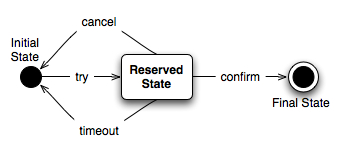
\includegraphics[scale=0.75]{images/TCC_general.jpg}
\caption{State machine representing a generic resource that implements the Try-Cancel/Confirm protocol}
\label{tcc-general}
\end{figure}
This protocol meets the need of industry, which has shown that transactions need not to be invasive. This in particular refers to the complexity in the design that might be introduced to create services that can participate in a transaction. With TCC's approach, we have loose coupling among resources: participating services are unaware of the fact that they are part of a global transaction. Indeed, the individual participating services do not need to have additional knowledge or implement any extra protocol besides the one they already support. \\
Also, with this solution we automatically avoid the use of an explicit transaction context, which is widely adopted in distributed transaction protocols. This is one of the most important requirements to ensure loose coupling.\\

\subsection{The protocol}
Before showing the protocol itself, let's define the transaction more formally:
\begin{theodef}
\label{transaction-definition}
A REST-based transaction T (e.g., purchasing two books) is a number of invocations $R_i$ (e.g., purchasing individual books) across REST-ful services $S_i$ (e.g., amazon.com and bookfinder.com) that need to either confirm altogether or cancel altogether. In other words: either all $R_i succeed$ via an explicit confirmation $R_i,confirm$ (e.g., by paying for the book) , or all $R_i$ cancel but nothing in between.
\end{theodef}

\subsubsection{Happy path}
\begin{enumerate}
\item A transactional workflow T goes about interacting with multiple distinct RESTful service APIs $S_i$
\item Interactions $R_i$ may lead to a state transition of the participating service $S_i$ identified by some URI - this URI corresponds to $R_i,confirm$
\item Once the workflow T successfully completes, the set of confirmation URIs and any required application-level payload is passed to a transaction service (or coordinator)
\item The transaction service then calls all of the $R_i,confirm$ with an idempotent PUT request on the corresponding URIs with the associated payloads
\end{enumerate}

The protocol (shown in \ref{tcc-overview}) guarantees atomicity because each service receives either a consistent request for cancel or to confirm. Moreover, all of them terminate their business transactions in the same way. Note that {\tt PUT} and {\tt DELETE} are idempotent actions, therefore we can assume $R_i,confirm$ is idempotent too. 

\begin{figure} [ht]
\centering
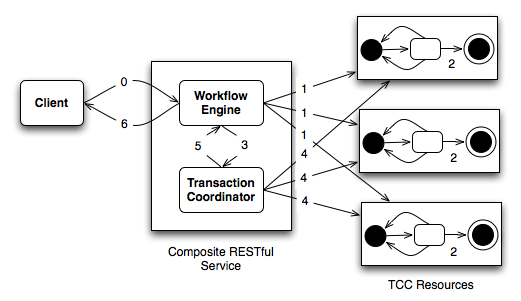
\includegraphics[scale=0.75]{images/TCC_overview.jpg}
\caption{Protocol architecture in the Happy Path case}
\label{tcc-overview}
\end{figure}

\subsubsection{Sad path}
The protocol looks very simple. How can this work in the presence of failure? This section will show what can go wrong and how can it recover from failures. We assume that each party is able to restore its own durable state, so we focus on the recoverability of the atomicity property across all parties.\\
We define recovery as follows:
\begin{enumerate}
\item Checking the state of a transaction after node failure followed by restart, or
\item Checking the state of a transaction triggered by timeout
\end{enumerate}
The recovery is performed by both the coordinator service and the participant services. The first one is expected to recover all the transactions he knows: if there were some pending transactions (waiting for a confirm action) we expect it to recover them all. On the other hand, the services want to recover the transactions because they want to release the reserved resources as early as possible.\\
As for the participant services, each participating service $S_i$ does the following:\\
\begin{enumerate}
\item For recovery before step 2, do nothing. 
\item For recovery after step 4: do nothing. 
\item For recovery in between steps 2 and 4: execute $R_i,cancel$ autonomously (This can be triggered by a timeout).
\end{enumerate}

For the coordinator things are a bit different. The most problematic failures are those happening during step 4. We want all the participants to arrive at the same end state for transaction T; step 4 involves multiple participants that are not aware that they are part of a transaction, so a failure here could be problematic.
\begin{enumerate}
\item For recovery before step 2, do nothing. 
\item For recovery between steps 2 and 4: do nothing. 
\item For recovery after step 4: do nothing. 
\item For recovery during step 4: retry $R_i,confirm$ with each participating service $S_i$. Since $R_i,confirm$ are performed using idempotent methods, they may be retried as many times as necessary. Note: this requires the coordinator to durably log all participant information before starting step 4.
\end{enumerate}

\begin{figure} [ht]
\centering
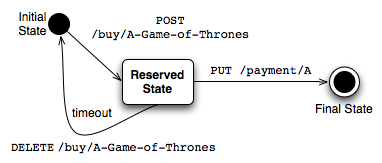
\includegraphics[scale=0.75]{images/TCC_booksExample.jpg}
\caption{Example of a book reservation.}
\label{tcc-bookexample}
\end{figure}

\subsection{Guaranteeing atomicity}
\label{tcc-guaranteeing-atomicity}
Even with failures, we can still (eventually) preserve atomicity. In fact, given enough time, the global transaction T will be finally confirmed everywhere or cancelled everywhere (or nothing happened). If we take a look at the protocol steps, we can prove that either all $R_i$ are confirmed or all are cancelled. More in details:
\begin{enumerate}
\item If there are no failures, then steps 1-4 run through and each $R_i$ will have been confirmed.
\item For any failures before step 2, no $R_i$ exists, meaning that nothing has happened.
\item For any failures during or after step 2 but before step 4: all $R_i$ will eventually be cancelled autonomously by each $S_i$.
\item For any failures during step 4: the coordinator will retry each $R_i$,confirm until it succeeds. Because confirmation is idempotent, this will eventually succeed.
\item For any failures after step 4: all $R_i,confirm$ have been done, so we already have atomicity and no action is required.
\end{enumerate}
\subsubsection{Saddest path}
Although everything seems fine and the protocol seems bullet-proof, there is one weak point in our proof of atomicity. During step 4, while the coordinator is confirming transactions, it may happen that some services $S_i$, that still has transactions that need to be confirmed, time out and cancel transactions on their own. In the worst case this means that some transactions will be confirmed and some will cancel, effectively breaking atomicity. This is what is called a \textit{heuristic exception}.\\
In the world of atomicity, there has been a lot of interesting work, but the most important result is that a perfect solution is not possible. In practice, there will always be a possibility that at least one participating service (or node) is unaware of the outcome of the global distributed transaction.\\
To avoid this problem it's very important to tune correctly the timeouts at the services side. If the timeout is too small (that is, resources are kept in a reserved state for a small amount of time) a client will find hard to confirm something in that small time slot, and may happen to have timeouts before and during step 4. On the other hand services want to have a timeout as small as possible, because they don't want resources to be kept in a reserved state for too long. This is mostly a matter of tuning, depending on which resources is the service offering and how many clients may be interested in those. We will explore this dimension in a later chapter.\\
The next chapter will dive into the architecture of how TCC can be implemented. It will especially focus on the $4+1$ architectural views.